
\documentclass{template/socthesis}

%\usepackage[left=35mm, right=30mm]{geometry}
\usepackage{subcaption}

\graphicspath{ {./images/} }

\addbibresource{sources.bib}

% Title Page
\titlesk{BrailleFeeder - pomôcka pre zrakovo postihnutých}
\school{Stredná odborná škola}
\address{Športová 675, 916 01 Stará Turá}
\author{Juraj Kulich}
\mentor{}
\field{18}


\begin{document}
	
\maketitle
\makecopyrightstatement{V Novom Meste nad Váhom}
\makethanks{Ďakujem svojmu spolužiakovi Romanovi Mariančíkovi za obetavú pomoc, podmetné  pripomienky a nekonečnú trpezlivosť, ktorú mi počas práce poskytoval.}

\tableofcontents

\chapter*{Úvod}
\addcontentsline{toc}{chapter}{Úvod}
V roku 2015 malo približne 441 milónov ľudí zrakové postihnutie. Z toho bolo 36 milónov ľudí slepých \cite{bourne2017magnitude}. Takíto ľudia môžu použiť namiesto klasického textu Braillovo písmo, avšak drvivá väčšina pomenovaní a názvov je v klasickom písme. Takisto nikde nenájdeme noviny v Braillovom písme.

Momentálne nájdeme veľmi málo interaktívnych pomôcok pre takýchto znevýhodnených ľudí. Telefóny môžu používať iba pomocou tzv. funkcie čítanie obrazovky, ktorá im číta obsah obrazovky. Táto funkcia je dobrá, ale pre určité úkony to môže byť zbytočne zdĺhavé a neintuitívne. Takisto na nej nenájdeme manuálny výstup. 


Aplikácia beží na systéme Android. Na tomto systéme beží celosvetovo už cez 2 miliardy aktívnych zariadení \cite{ng_2017}. Náš systém beží na minipočítači, na ktorom je platforma Android Things, ktorá je taktiež založená na Androide. Z toho dôvodu môžeme našu aplikáciu implementovať aj na mobilné zariadenia, na ktoré však nemôžeme pripojiť periférie a tak je funkčnosť obmedzená.
\newpage

\chapter*{Cieľ a metodika práce}
\addcontentsline{toc}{chapter}{Cieľ a metodika práce}
Cieľom tejto práce je teda prototyp, ktorý úmožní čítať články nevidiacim, vypočuť si články, rozpoznať objekty zo snímky vytvorenej fotoaparátom. Tento prototyp môže teda slúžiť ako pomoc nevidiacim.

Táto práca začína dvoma teoretickými kapitolami. Prvá sa zaoberá vo všeobecnosti Braillovým písmom a druhá približuje základné zásady Android systému. Tretia kapitola popisuje architektúru a funkčnosť zariadenia. Samotnú implementáciu opisuje štvrtá kapitola. V poslednej kapitole sú opísané výsledky testovania a prezentovaná celková úspešnosť zariadenia. V závere nájdeme zhodnotené dosiahnuté výsledky a návrhy na možné vylepšenia. 
\newpage

\chapter{Braillovo písmo}
Braillovo písmo je druh písma určeného pre nevidiacich a slabozrakých. Funguje na princípe vyvýšených bodov, ktoré sa dajú čítať hmatom. Zhotovil ho slepý Louis Braille pôvodne z vojenského písma. 

Jedno písmeno Braillovho písma tvorí obdĺžnik bodov s dvoma stĺpcami a troma riadkami, ktorý sa nazýva braillovská bunka. Písmeno Braillovho písma je vo veľkosti rozmeru ukazováka, keďže na brušku ukazováka je najcitlivejší prah hmatu.
Na bunke je možné vytvoriť 64 znakov vrátane prázdnej bunky, ktorá tvorí medzeru. 
Základnú sadu tvoria písmená malej abecedy a interpunkčné znamienka. Čísla a veľké písmená sa tvoria pomocou prefixov.  Napríklad písmeno „c”,  „C” a číslo 3 sa zapíšu tým istým znakom, na rozoznanie sa však používa prefixový znak (Obr. 1.1).

\begin{center}
	\begin{figure}[htp]
		\centering
		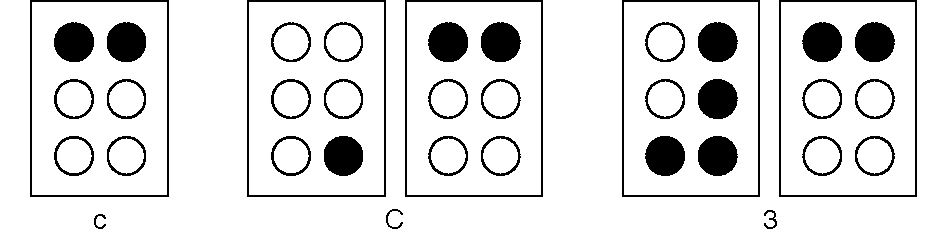
\includegraphics[scale=0.8]{braille}
		\caption{Príklady písmen s ukážkou prefixov}
	\end{figure}
\end{center}

\section{Rôzne normy a formy Braillovho písma}
Najpoužívanejšie formy písma sa nazývajú Grade 1 a Grade 2. Vo forme Grade 1 (plnopis) sa slová prepisujú znak po znaku zatiaľ čo pri forme Grade 2 (skratkopis) dokáže jeden znak znamenať viacero hlások. Skratkopis sa u nás nepoužíva ale je používaný najmä v anglicku.  

\begin{center}
	\begin{figure}[htp]
		\centering
		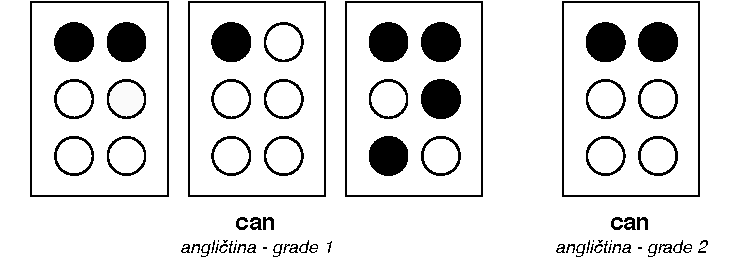
\includegraphics[scale=1]{brailleGrades}
		\caption{Porovnanie anglického slovesa „can” vo forme 1 a 2}
	\end{figure}
\end{center}

Jedným z problémov Braillovho písma je nejednotnosť noriem, ktoré sa výrazne odlišujú. Napríklad medzi českou a slovenskou formou je už v základných písmenách abecedy 7 rozdielov \cite{braille-wiki}. Z dôvodu jednoduchosti a použitia aj slovenského jazyka v ktorom sa skratkopis nepoužíva, v tejto práci používame normu \textit{grade 1}. 


\newpage
\chapter{Android OS}
Android je open source operačný systém pre mobilné zariadenia vyvíjaný spoločnosťou Google. Je postavený na jadre Linuxu. V tejto kapitole si ukážeme vlastnosti  a princípy tohto systému a spôsoby tvorby aplikácii pre tento systém.

\section{Android Things OS}
Android Things je zjednodušená verzia operačného systému Android prispôsobená pre IoT zariadenia. Je navrhnutý tak aby fungoval v inteligentných zariadeniach, napríklad termostatoch alebo kamerách.

\section{Základné princípy Android systému}
V tejto kapitole si priblížime potrebné súčasti pre programovanie pre Android.

\subsection*{Architektúra systému Android}

Architektúra systému Android je rozdelená do niekoľkých vrstiev (Obr. 2.1) pričom každá vrstva využíva služby vrstvy pod ňou. 
\begin{center}
	\begin{figure}[htp]
		\centering
		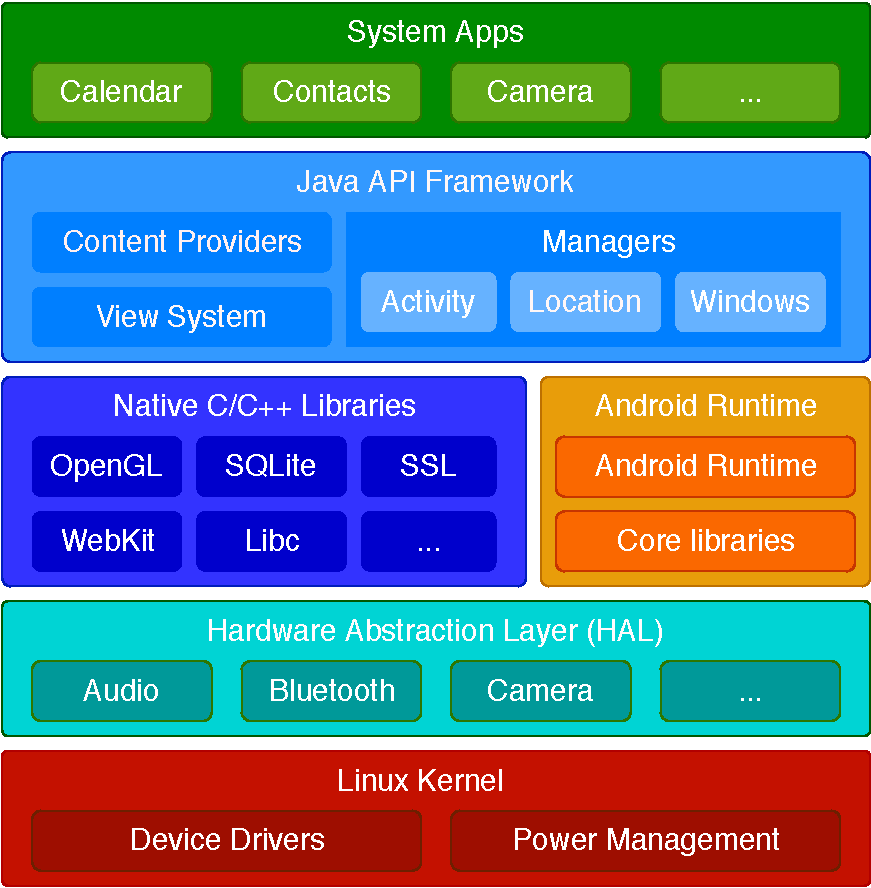
\includegraphics[scale=0.80]{android_architecture}
		\caption{Architektúra systému Android}
	\end{figure}
\end{center}

Vrstvy začiatkom od spodnej sú \cite{gandhewar2010google}\cite{androiddevelopers}:
\begin{itemize}
	\item Linux Kernel -- Jadro systému, ktoré poskytuje systémové služby ako sú bezpečnosť, správa pamäte, procesov, sietí a driverov. Slúži taktiež ako abstraktná vrstva medzi hardvérom a softvérom.  
	\item Hardware Abstraction Layer (HAL) -- Hardvérová abstraktná vrstva, ktorá poskytuje štandardné rozhrania vyššej vrstve. Skladá sa z rôznych knižníc, z ktorej kazdá implementuje rozhranie pre špecifický komponent, napríklad kameru alebo Bluetooth.
	\item Libraries -- Obsahuje knižnice písané v jazykoch C a C++. Sú volané cez Java rozhranie. Obsahujú knižnice pre zobrazovanie okien, jadrá pre 2D alebo 3D grafiku, kodeky ako MP3 alebo MPEG-4, SQL databázu alebo WebKit - renderovacie jadro pre prehliadače. 
	\item Android Runtime -- Obsahuje základné knižnice, ktoré poskytujú väčšinu funkcií dostupných v knižniciach jazyka Java. Ďalej obsahuje aplikačný virtuálny stroj Dalvik. 
	
	Virtuálny stroj \textit{Dalvik} -- Vytvára runtime prostredie pre Java aplikácie. Java aplikácie sa najprv prekladajú do bajtkódu pre virtuálny stroj Java, ten sa prekladá do bajtkódu Dalvik a ukladá do súborov .dex - Dalvik Executable a .oed - Optimized Dalvik Executable. Tieto súbory sú menšie a efektívnejšie na Android zariadeniach, ktoré majú slabší procesor a pamäť. Dalvik vytvára pre každú aplikáciu samostatnú inštanciu virtuálneho stroja.  
	 
	\item Java API Framework -- Obsahuje sadu funkcií v jazyku Java potrebných pre tvorbu mobilných aplikácií.
		\begin{itemize} 
		\item View System -- Poskytuje rozhranie pre stavbu užívateľského prostredia
		\item Resource Manager -- Poskytuje prístup k externým zdrojom ako sú reťazce, grafické prvky a súbory s~rozložením prostredia. 
		\item Notification Manager -- Poskytuje prístup k zobrazovaniu notifikáciam v stavovom riadku.
		\item Activity Manager -- Riadi životný cyklus aplikácie.
		\item Content Provider -- Umožňuje zdieľať dáta ostatným aplikáciam.
		\end{itemize}
	\item System Applications -- Je to najvyššia vrstva, ktorá poskytuje množstvo základných aplikácií ako sú email, SMS program, kalendár, aplikácie tretích strán a podobne.
\end{itemize}

\section{Tvorba aplikácií pre Android OS}
\subsection*{Softvérové nástroje}
Pre programovanie pre Android nám stačia nasledovné nástroje:
\begin{itemize}
	\item Java JDK -- Obsahuje základné nástroje na vývoj aplikácií pre Java platformu.
	\item Android SDK -- Poskytuje prístup ku knižniciam Androidu. Obsahuje debugger, Android knižnice, emulátor a dokumentáciu. 
	\item Android Studio -- Oficiálne vývojové prostredie pre Android. 
\end{itemize}

\subsection*{Android Manifest}
Základom každej aplikácie je súbor \textit{AndroidManifest.xml}. Je uložený v koreňovom priečinku každej aplikácie. Tento súbor poskytuje všetky dôležité informácie o aplikácii Android systému. Najdôležitejším je atribút \textit{package}, ktorý označuje unikátny názov aplikácie v Android systéme aj v obchode Google Play. Ďalšie dôležité informácie sú \cite{9781118387108}:
\begin{itemize}
	\item \textbf{Špecifikácie aplikácie} -- Špecifikuje samotné komponenty aplikácie ako sú aktivity \texttt{<activity>}, služby \texttt{<service>}, content providery \texttt{<provider>} a ďalšie. V tagu \texttt{<application>} ďalej nastavujeme meno aplikácie a ikonu aplikácie v Android zariadení. 
	
	V tagu samotnej aktivity nastavujeme meno triedy (parameter \texttt{android:name}), zobrazované meno aktivity (parameter \texttt{android:label}) a často tiež prvok \texttt{<intent-filter>}, ktorý špecifikuje, za akých podmienok sa spustí aktivita.
	
	Príklad špecifikácie aplikácie BrailleApplication, ktorá spustí aktivitu \textit{MainActivity} po spustení aplikácie:
	
	\begin{verbatim}
		<application
		  android:name=".BrailleApplication"
		  android:label="Braille">
		
		  <activity android:name=".ui.main.MainActivity">
		    <intent-filter>
		      <action android:name="android.intent.action.MAIN"/>
		      <category android:name="android.intent.category.LAUNCHER"/>
		    </intent-filter>
		  </activity>
		</application>
	\end{verbatim}
	
	
	\item \textbf{Zoznam povolení} -- Špecifikuje zoznam povolení, ktoré aplikácia potrebuje na fungovanie. Bez potvrdenia povolenia užívateľom nemôže aplikácia použiť danú funkciu. Jedná sa napríklad o prístup k internetu, zápis do pamäte, prístup ku kamere a podobne.
	
	Príklad tagu na povolenie pre používanie internetu: \\
	\texttt{<uses-permission   android:name="android.permission.INTERNET" />
	}
	\item \textbf{Minimálna verzia systému} -- Určuje minimálnu verziu Android systému, potrebnú na správne fungovanie aplikácie. Verzie sa od seba môžu odlišovať novými triedami, metódami alebo parametrami. 
	
	Príklad tagu na nastavenie minimálnej verzie systému na verziu 25 (Android 7.1.1): \\
	\texttt{<uses-sdk android:minSdkVersion="25" />}	
\end{itemize}

\subsection*{Lokalizácia aplikácie}
Android funguje na zariadeniach v mnohých regiónoch. Aby sme nemuseli vyvíjať viac aplikácií s rôznymi jazykmi používame lokalizáciu. Lokalizácia sa stará o prispôsobenie textu, obrázkov, čísel alebo meny podľa regiónu použitia. 

Android na takéto zmeny používa prepínanie zdrojov. Zdroje môžu obsahovať rôzne nastavenia pre rôzne prípady ako napr. rozloženie prostredia pre zvislú polohu a horizontálnu polohu telefónu, rozdielne obrázky pre rôzne rozlíšenia, lokalizované reťazce pre rôzne jazyky, atď.

Základné zdroje nájdeme v zložke \texttt{/res/values}. V tejto zložke je automaticky vytvorený súbor \texttt{strings.xml}, ktorý obsahuje reťazce používané v prápade že nie je dostupná žiadna iná lokalizácia. Po pridaní slovenskej lokalizácie sa vytvorí nová zložka \texttt{/res/values-sk-rSK/strings.xml}. Akonáhle bude mať zariadenie nastavené slovenský jazyk, aplikácie bude používať zdroje zo slovenskej lokalizácie. V aplikácii tak nie je vhodné používať konštatné reťazce ale reťazce zo zdrojov. V našom prípade používame slovenskú lokalizáciu pre zvukový výstup zariadenia.

\subsection*{Práca s perifériami}
Pre prácu s perifériami slúži systémová služba \textit{PeripheralManager}. Pomocou tejto triedy dokážeme nastavovať a ovládať  GPIO piny. Taktiež obsahuje callback na prijímanie signálov z pinov.
\newpage

\chapter{Hardvérová architektúra zariadenia}
V tejto kapitole si ukážeme architektúru nášho zariadenia. Ukážeme si časti z ktorých sa skladá a ako prispievajú k správnej funkčnosti.

\section{Vývojová doska}
Mozog zariadenia tvorí HW platforma NXP i.MX7D. Táto platforma obsahuje množstvo zberníc a pinov na pripojenie rôznych zariadení. Tu využívame USB na pripojenie mikrofónu, RJ45/Wi-Fi na pripojenie k internetu, konektor na pripojenie fotoaparátu, 3.5mm jack na pripojenie audio zariadení a univerzálne piny GPIO na pripojenie ostatných potrebných periférií(tlačidlá, cievky, …).
Táto platforma má procesor ARM Cortex-A7 - 1GHz, 512MB pamäte RAM a 4GB internú pamäť. Fotoaparát sa pripája pomocou MIPI CSI rozhrania. Operačný systém tejto platformy je Android Things.

\begin{center}
	\begin{figure}[htp]
		\centering
		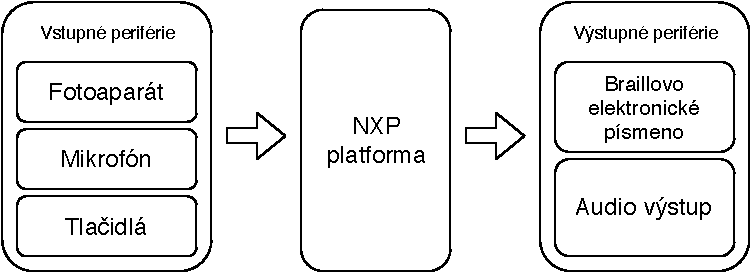
\includegraphics{brailleblock}
		\caption{Bloková schéma zariadenia}
	\end{figure}
\end{center}

\section{Časti elektroniky}
\subsubsection{Elektronické Braillovo písmeno}
Základným prvkom tejto vlastne vyrobenej periférie je 6 elektronicky ovládaných solenoidov usporiadaných do obdĺžnika - tvoria jedno Braillovo písmeno. V platforme sa články prekonvertujú do kombinácii núl a jednotiek, ktoré sa odosielajú na vstupy tohto zariadenia pomocou GPIO pinov, a podľa toho vytvoria vysúvaním dané písmeno. 

Solenoid je súčiastka, ktorej časť sa za pomoci magnetu a cievky dokáže vysúvať a zasúvať. Keďže naša platforma dokáže na jednom GPIO pine poskytnúť maximálny prúd okolo 20mA, napájanie je riešené pomocou externej batérie. Tým pádom potrebujeme 6 optočlenov a tranzistorov na zopínanie cievok.

\subsubsection{Batérie}
Slúžia na napájanie dosky a modulu s cievkami(Braillovo písmeno). Používame tri nabíjateľné 3400mAh 3.7V batérie typu 18650. Na napájanie dosky používame napäťový booster z 3.7V na 5V.

\subsubsection{GPIO piny}
General-purpose input/output - sú digitálne piny, ktoré dokážu slúžiť aj ako vstupy aj výstupy podľa potreby. Používame ich ako výstupy pre posielanie impulzov do cievok a ako vstupy pri tlačidlách. 

\subsubsection{USB vstup}
Slúži na pripojenie USB mikrofónu.

\subsubsection{3.5mm jack}
Slúži na pripojenie audio zariadení pre hlasový výstup.

\section{Režimy použitia}
Naše zariadenie dokáže pracovať	 vo viacerých režimoch:
\begin{enumerate}
\item Prehrávanie článkov na Braillovom písmene -- článok sa rozdelí na písmená a každé písmeno sa skovertuje na príslušný kód, podľa ktorého sa zobrazí výstupe.
\item Prehrávanie článkov cez reproduktor.
\item Vstup pre základné úkony pomocou tlačidiel. 
\begin{itemize}
\item prepínanie článkov
\item nastavenie hlasitosti
\item nastavenie rýchlosti prepínania Braillovho písma.
\end{itemize}
\item Vstup pre rozšírené úkony cez mikrofón (hlasové ovládanie) -- hlasové ovládanie je z dôvodu gramatickej nestálosti slovenského jazyka dostupné iba v anglickom jazyku.
\begin{itemize}
\item prepínanie článkov dopredu/dozadu
\item nastavenie hlasitosti na presnú hodnotu
\item určenie kategórie vyhľadávaných článkov 
\item vyhľadávanie článkov o konkrétnej téme
\item uloženie článkov do offline pamäte
\item načítanie uložených článkov
\item vytvorenie snímku
\item zmena jazyka prostredia do slovenského jazyka
\item pomocný príkaz pre nápovedu
\end{itemize}
\end{enumerate}

\chapter{Softvérová architektúra zariadenia}
Táto kapitola popisuje softvérovú časť zariadenia, použité technológie a zámery.

\section{Použité technológie}
Na vývoj hlavného programu bol použitý jazyk Java z dôvodu predchádzajúcich skúseností s týmto jazykom a veľmi rozšírenou komunitou. Pri programovaní sme sa snažili dodržať všetky koncepty objektovo-orientovaného programovania ako sú dedičnosť, abstrakcia, zapuzdrenosť a polymorfizmus. \\

Použili sme oficiálne vývojové prostredie od Googlu - Android Studio. Toto prostredie je postavené na vývojovom prostredí IntelliJ IDEA a podporuje dopĺňanie príkazov, refaktoring alebo analýzu kódu. Toto prostredie obsahuje aj emulátor, ktorý slúži ako virtuálne Android zariadenie. Na ukladanie údajov používame SQL databázu.

\subsection*{Použité knižnice}
\subsubsection{Butterknife}
Knižnica Butterknife generuje k prvkom z rozhrania(napr. tlačidlo) štandardizovaný kód, čím nám skracuje dĺžku kódu a robí ho prehľadnejším.
\subsubsection{OkHttp}
Knižnica OkHttp slúži na posielanie a prijímanie HTTP a HTTP/2 požiadavok a prijímanie/spracovávanie odpovedí zo servera.
\subsubsection{Retrofit}
Retrofit je REST (Representational State Transfer) klient s typovou kontrolou. REST je rozhranie, ktoré definuje metódy pre prístup k dátam - vytvoriť, zmazať, upraviť, získať. Pomocou neho získavame dáta z internetu a ukladáme do našich Java tried.
\subsubsection{Room}
Poskytuje abstraktnú vrstvu nad SQL databázou, umožňuje lepší prístup k databáze použitím menšieho množstva kódu a overuje dotazy na databázu.
\subsubsection{Cloud Vision API}
Umožnuje zistiť obsah z fotografie. Detekuje skupiny objektov a vecí (napr. rastliny, zvieratá, …) a extrahuje tlačený text.
\subsubsection{Cloud Speech-To-Text API}
Konvertuje audio do textu. Slúži na hlasové ovládanie.
\subsubsection{Cloud Translation API}
Poskytuje rozhranie na preklad textu. V našom prípade z angličtiny do slovenčiny. Toto API zatiaľ nepodporuje Android a preto posielame požiadavku na server s textom, ktorý chceme preložiť.

\chapter{Konštrukčná časť}
\newpage



\chapter*{Výsledky práce}
\addcontentsline{toc}{chapter}{Výsledky práce}
\newpage
\chapter*{Diskusia}
\addcontentsline{toc}{chapter}{Diskusia}
\newpage
\chapter*{Záver}
\addcontentsline{toc}{chapter}{Záver}
\newpage
\chapter*{Zhrnutie}
\addcontentsline{toc}{chapter}{Zhrnutie}
\newpage

\printbibliography[title=Zoznam použitej literatúry]
\newpage

\chapter*{Zoznam použitých skratiek a symbolov}
\addcontentsline{toc}{chapter}{Zoznam použitých skratiek a symbolov}
\begin{table}[!ht]
	\begin{tabular}{lll}
		\textbf{skratka} & \textbf{celý názov} & \textbf{vysvetlenie} \\
		IoT              & Internet of Things  & \makecell{Označuje zariadenia	so sieťovou konektivitou\\ umožňujúce vzájomné prepojenie a výmenu dát}       
	\end{tabular}
\end{table}

\end{document}          
